\chapter{Diagramma delle classi} \label{cap2}
\def\baselinestretch{1.66}
Di seguito vengono illustrati i \textbf{diagrammi delle classi} che fanno uso di specifici pattern. Per quanto riguarda le servlet, poich\'e queste hanno tutte le stesse \textbf{signature} si \`e deciso di mostrare solamente
quelle che mostrano le informazioni alle views, piuttosto che elencare tutti i controller delle
\textbf{rotte}\footnote{In ambito web le rotte non sono altro che le risorse della url}.
\section{Servlet come controller}
\begin{figure}[ht]
    \centering
    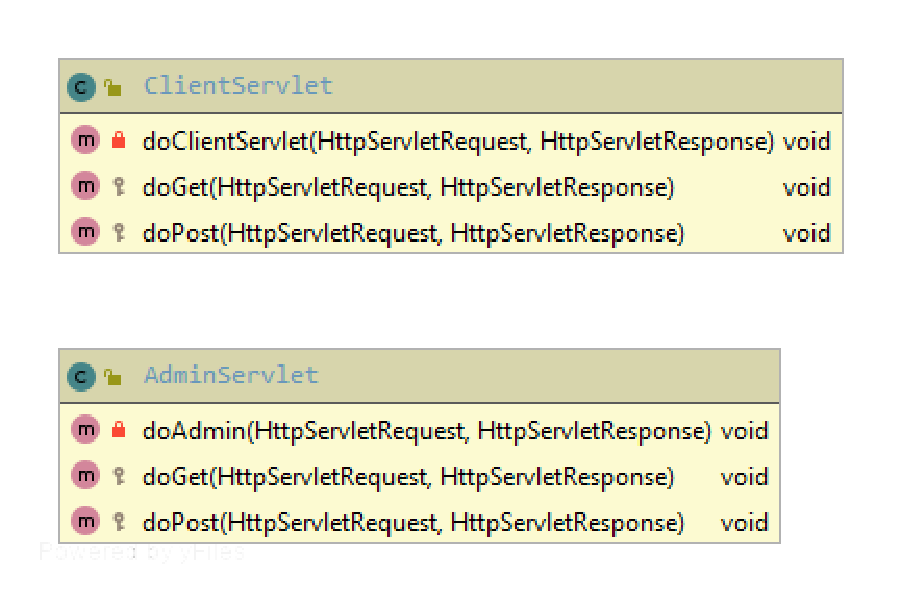
\includegraphics[scale=0.6]{img/servlet.eps}
    \caption{Servlet principali per le informazioni da passare alle views.}
\end{figure}
\newpage
\section{Template Method e Singleton}
Metodi per le operazioni del database creati con il template method e singleton. L'unica
classe usata per interrogare il database sar\`a \textbf{GenericDao} che \`e una classe templata.
\begin{figure}[ht]
    \centering
    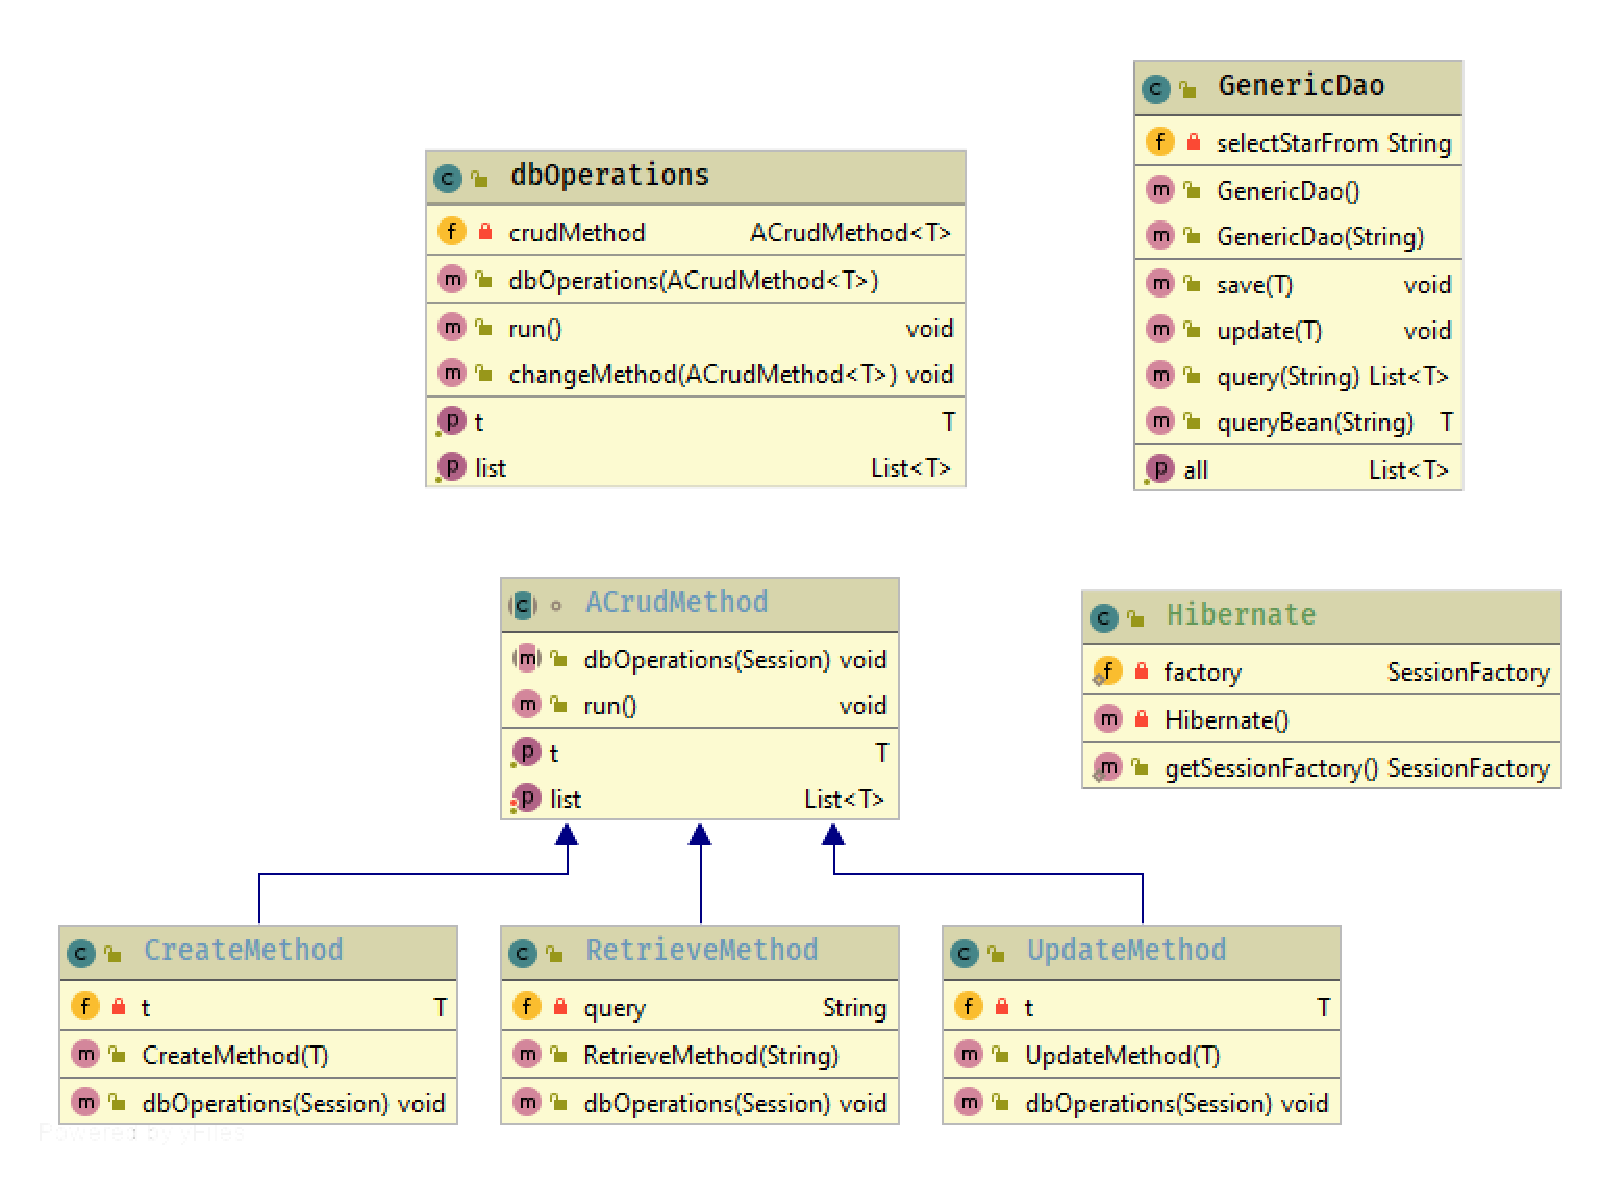
\includegraphics[scale=0.6]{img/tm.eps}
    \caption{Diagramma dei metodi templati.}
\end{figure}
\newpage
\section{Java Bean}
Principali Java Bean usate per "mappare" le entit\`a del database
\begin{figure}[ht]
    \centering
    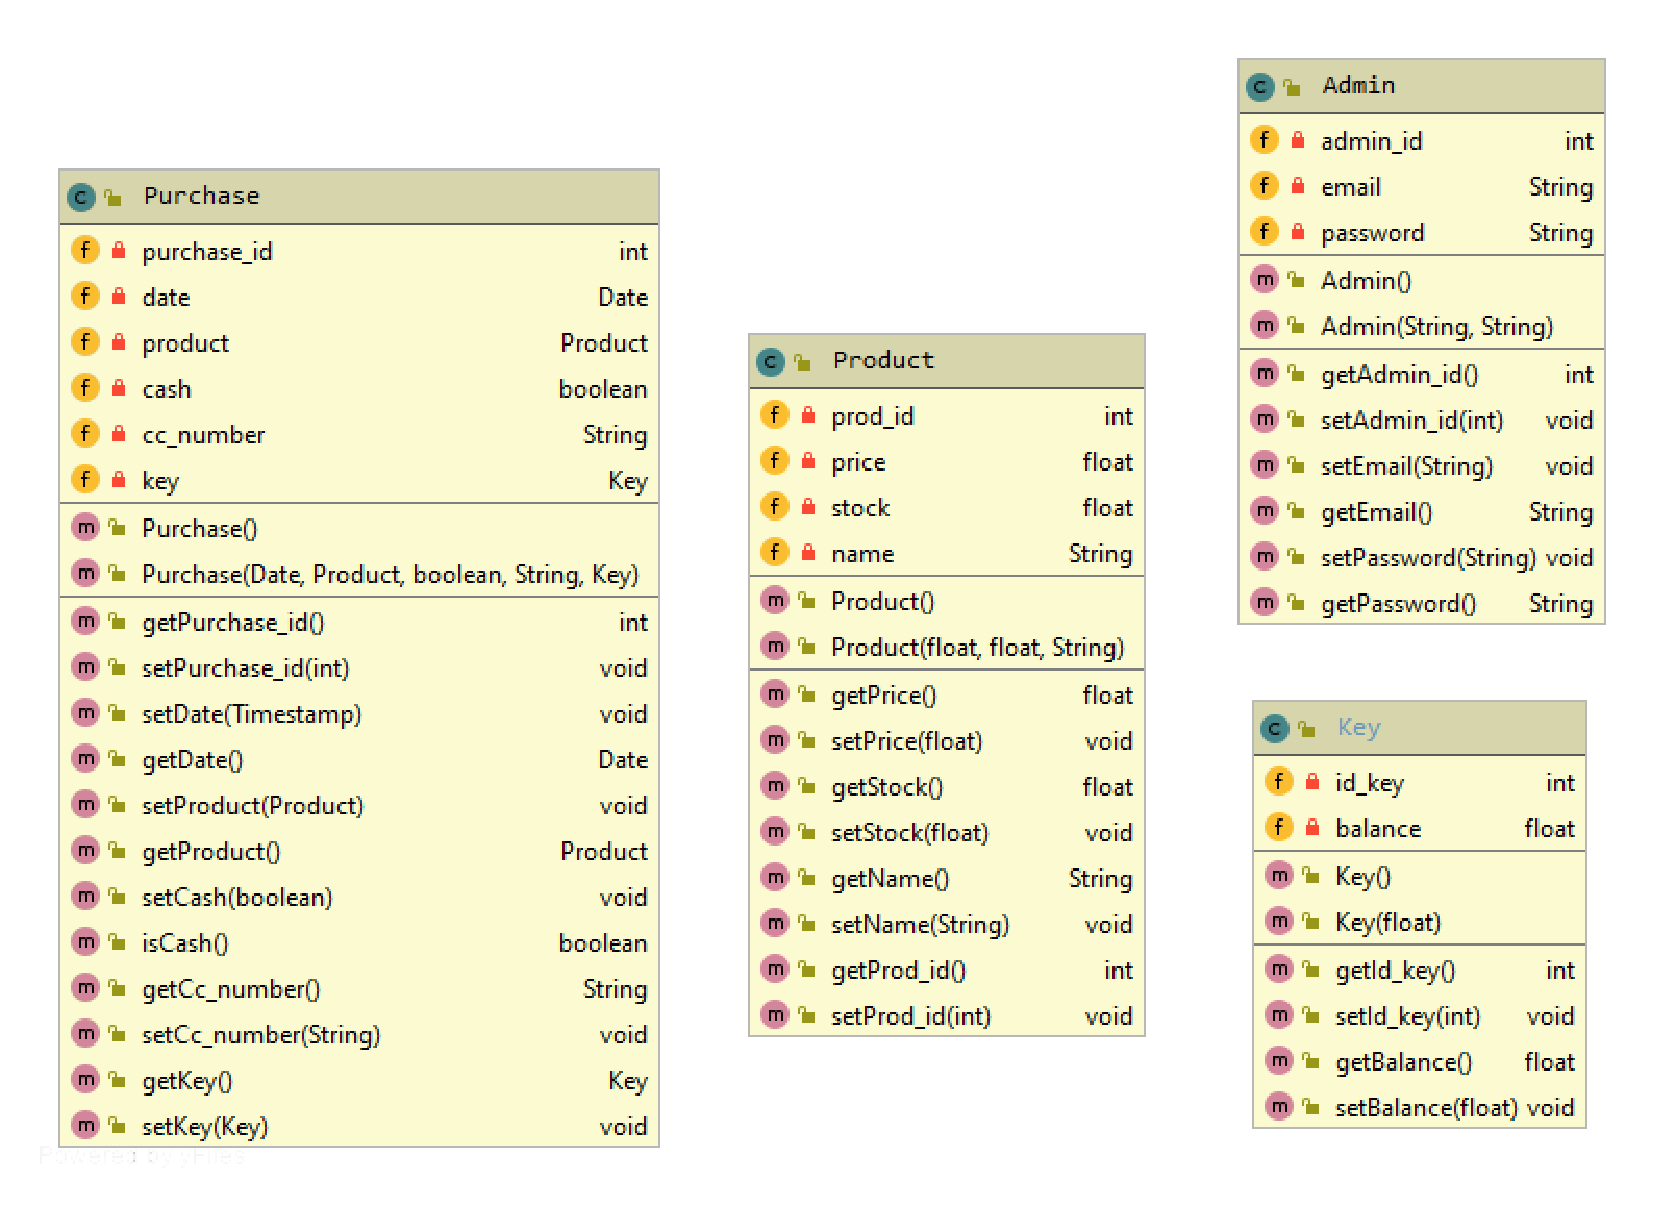
\includegraphics[scale=0.5]{img/javabean.eps}
    \caption{Java bean.}
\end{figure}
\newpage
\section{Chain of Responsibility}
Controllo dei metodi di pagamento tramite catena di responsabilit\`a.
\begin{figure}[ht]
    \centering
    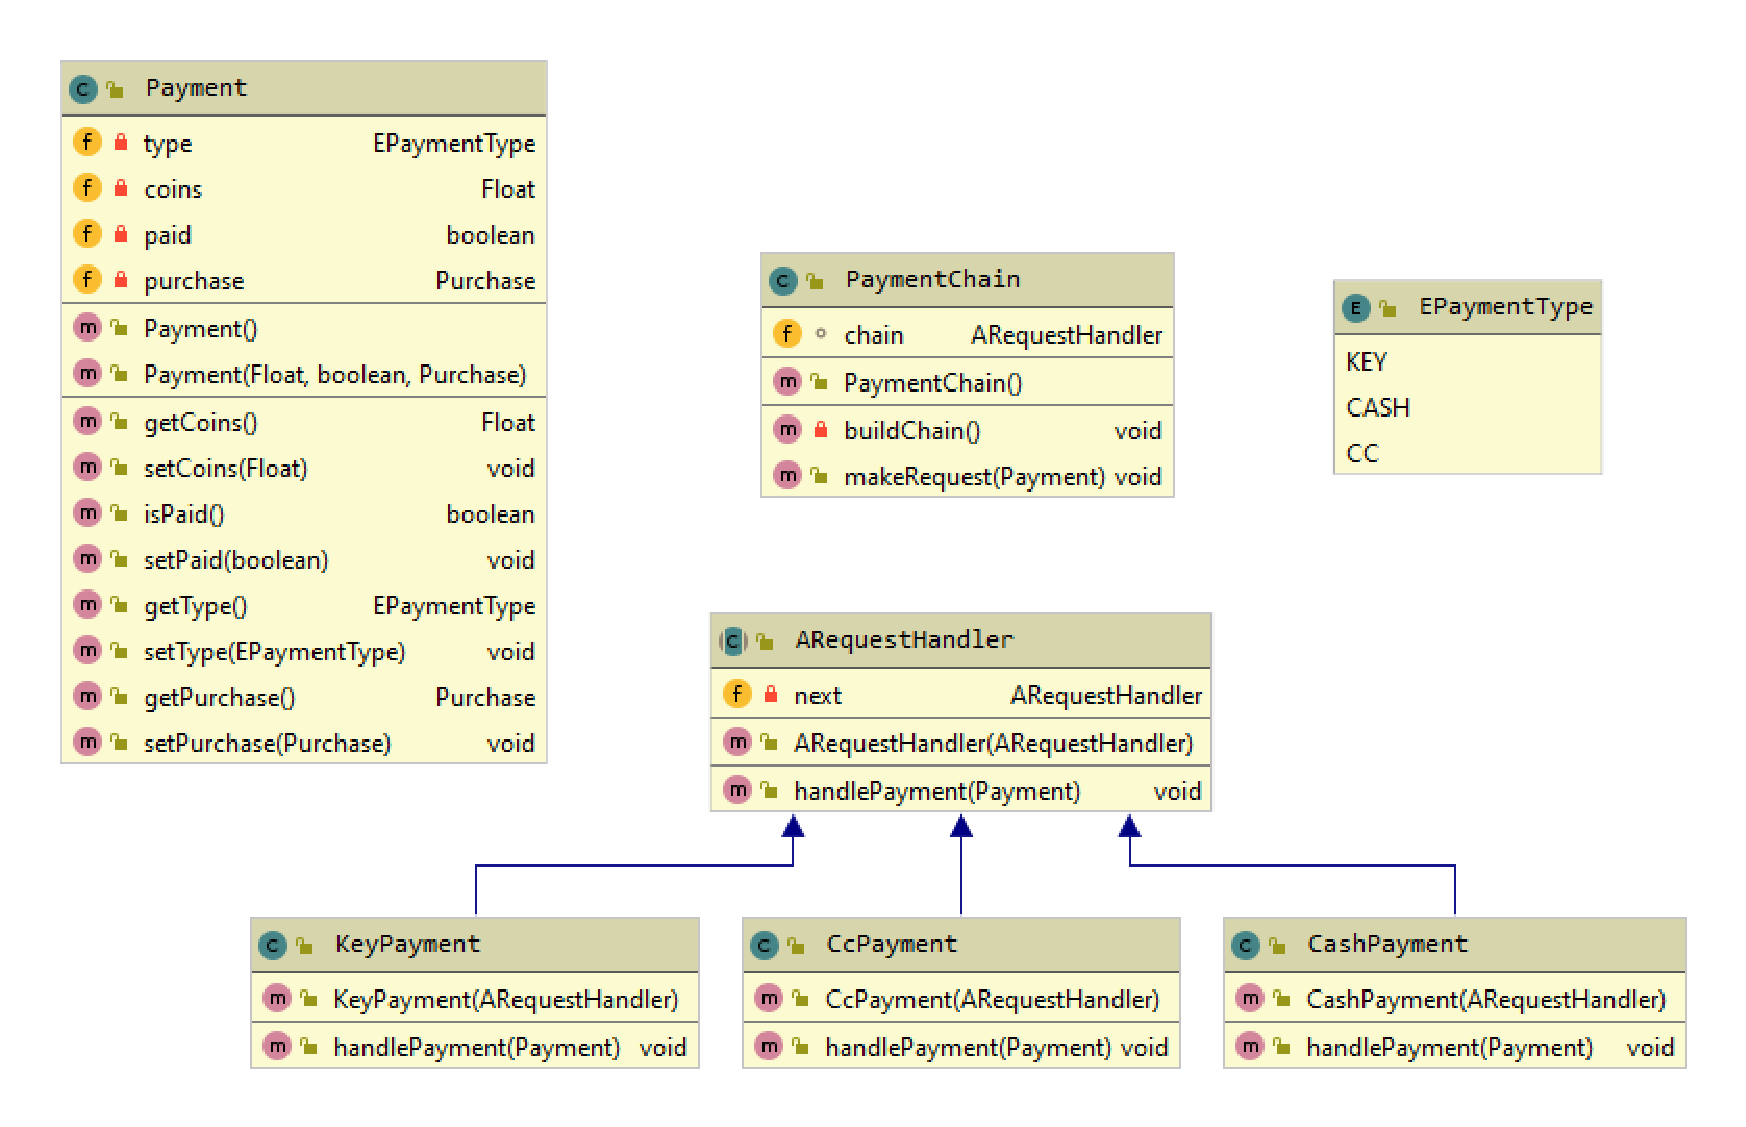
\includegraphics[scale=0.5]{img/cor.eps}
    \caption{Diagramma della Chain of Responsibility.}
\end{figure}
\newpage
